
 Consider a plane  curve $\mathcal{C}(t)=[x(t),y(t)]$ defined by a support function $h$:

\begin{align}
x(t)=&h(t)\cos t-h'(t)\sin t \label{eqn:support}\\
y(t)=&h(t)\sin t+h'(t)\cos t \nonumber
\end{align}
%

\begin{remark*} In terms of a support function $h(t)=\sqrt{a^2\cos^2{t}  + b^2\sin^2{t}}$
the  ellipse is parametrized by:
\[  \left[ \frac{a^2\cos{t} }{ \sqrt{a^2\cos^2{t}  + b^2\sin^2{t}}}, \frac{b^2\sin{t}}{\sqrt{a^2\cos^2{t}  + b^2\sin^2{t}}} \right]\]
\end{remark*}

Let $M=(x_0,y_0)$ be a fixed point. Referring to Equation~\ref{eqn:support}, the pedal of $M$ is given by

\begin{equation}\label{eq:pedal-suporte}
 P_M(t)= [  x_0 \sin^2 t + \left( h(t) -y_0\sin
 t    \right) \cos t, \left( h(t) -{  x_0}\,\cos t  
   \right) \sin t +   y_0\cos^2 t ].
\end{equation}


The contrapedal of $M$ (intersection of the line $M+s \mathcal{C}'(t)$ and the normal line $\mathcal{C}(s)+u\mathcal{C}'(t)^{\perp}$) is given by

\begin{equation}\label{eq:contrapedal-suporte}
C_M(t)=  [ x_0  \cos^2t   +y_0\cos t
 \sin t -h'(t) \sin t , y_0 \sin^2t
 +x_0\cos t \sin t 
	 + h'(t) \cos t]
.
\end{equation}

Below is a generalization of Corollary~\ref{cor:area-diff}.


\begin{proposition}
For all smooth curves, the following holds:
	\[A(P_M)-A(C_M)=A(\mathcal{C})\]
	\label{prop:darea}

\end{proposition}

\begin{proof}
Obtain the signed areas for the above curves above via integration by parts of  Equation~\ref{eqn:area}. Algebraic manipulation yields the claim.
In fact, 
{\small  
\begin{align}
A(P_M)=& \frac{\pi}{2}(x_0^2+y_0^2)- \left(\int_0^{2\pi}\!\!\!\!\!\!h(t)\cos t dt\right) x_0- \left(\int_0^{2\pi}\!\!\!\!\!\!h(t)\sin t dt \right) y_0+\frac{1}{2}  \int_0^{2\pi}\!\!\!\!\!\!h(t)^2 dt\nonumber \\
A(C_M)=& \frac{\pi}{2}(x_0^2+y_0^2)- \left(\int_0^{2\pi}\!\!\!\!\!\!{h(t)\cos{t}dt}\right) x_0- \left(\int_0^{2\pi}\!\!\!\!\!\!h(t)\sin t dt \right) y_0+\frac{1}{2}\int_0^{2\pi}\!\!\!\!\!\!h^\prime(t)^2 dt \label{eqn:apm-acm}\\
A(\mathcal{C})=& \frac{1}{2}\int_0^{2\pi}\!\!\!\!\!(h(t)^2-h^{\prime}(t)^2)dt\nonumber
%
\end{align}
}
\end{proof}

%\begin{corollary}
%For any plane curve with vanishing signed area, $A(P_M)=A(C_M)$
%\end{corollary}

\begin{corollary} The family of isocurves of $A(P_M)$ and $A(C_M)$ are circles centered at
	
\begin{align*}
K_0=\left[  	\frac{1}{\pi} \int_0^{2\pi}\!\!\!\!\! h(t)\cos t \,dt,	\frac{1}{\pi} \int_0^{2\pi}\!\!\!\!\! h(t)\sin t \, dt\right]
\end{align*}
	
	
\end{corollary}
 
\begin{proof}  Consider the mean $K_0=\frac{1}{2\pi}\int_0^{2\pi}\mathcal{C}(t)dt$ of the curve $\mathcal{C}$ given by Equation \eqref{eqn:support}. Integration by parts leads to the result stated. Expressions of the areas $A(P_M)$ and $A(C_M)$ given in Equation \eqref{eqn:apm-acm} shows that the isocurves are cirles centered at $K_0$.
\end{proof}

\begin{remark}
For convex curves,  $K_0$ coincides with the   centroid of Steiner $K$ given by Equation \eqref{eqn:steiner-k}. In fact, using the parametrization  of the curve $\mathcal{C}$ given by Equation \eqref{eqn:support} it follows that
$ds= |h(t)+h''(t)|dt$ and $k(t)=1/(h(t)+h''(t))$. Integration by parts leads to the result.
\end{remark}

\begin{proposition} Let $P_{ {\theta }M}$ be the pedal of $M$ with respect to the curve $\mathcal{C}_\theta$.  For any convex curve $\mathcal{C}$ we have that:
	\[A(P_M)-A(P_{ {\theta }M})=\sin^2\theta A(\mathcal{C})\]
	
	\end{proposition}

\begin{proof} Similar to   that of Proposition \ref{prop:darea}.
\end{proof}

Referring to Figure~\ref{fig:interp-concave} and generalizing Proposition~\ref{prop:interpol}:

%\begin{proposition}
%\label{prop:amu}
%Let $\mathcal{C}_\mu=\mu P_M+(1-\mu)C_M$
	
%	Then, for $\mu\ne \frac{1}{2}$  the area isocurves of $\mathcal{C}_\mu$ are circles centered on $K$.
	
%	For  $\mu=\frac{1}{2}$,  the area isocurves of $\mathcal{C}_{\frac{1}{2}}$ are independent of the point $M$.
%\end{proposition}

%\begin{proof} Similar to the that of Proposition \ref{prop:darea}.
%	In fact, 
%	\begin{align*}
%	\mathcal{C}_\mu=&(2\mu-1)^2\left[   \frac{\pi}{2}(x_0^2+y_0^2)- \left(\int_0^{2\pi}\!\!\!\!\!\!h(t)\cos t dt\right) x_0- \left(\int_0^{2\pi}\!\!\!\!\!\!h(t)\sin t dt \right) y_0\right]\\
%	+&\frac{\mu^2}{2}  \int_0^{2\pi}\!\!\!\!\!\!h(t)^2 dt +\frac{(3\mu-1)(\mu-1)}{2}  \int_0^{2\pi} \!\!\!\!\!\!h^\prime(t)^2 dt.
%	\end{align*}
	
%	For $\mu=\frac{1}{2}$, it follows that $\mathcal{C}_{\frac{1}{2}}=\frac{1}{2}(M+\mathcal{C})$.\end{proof}

%\begin{corollary}
	
%	\begin{align*}
%	A(\mathcal{C}_\mu)=&(2\mu-1)\left( \mu A(P_M)+(1-\mu)A(C_M)\right)\\
%	+&\frac{\mu}{2}  \int_0^{2\pi}\!\!\!\!\!\!h(t)^2 dt+\frac{(\mu-1)(2\mu-1)}{2} \int_0^{2\pi}\!\!\!\!\!\! h^\prime(t)^2 dt  
%\end{align*}
%\end{corollary}

\begin{proposition}
\label{prop:amu-concave}
For any smooth regular closed curve $\mathcal{C}$ with non-zero rotating index, the isocurves of $A(\mathcal{C}_\mu)$ are circles centered on $K$.
In fact, \[A(\mathcal{C}_\mu) =(1-2\mu)[(1-\mu) A(P_M)-\mu A(C_M)]+\mu(1-\mu)A(\mathcal{C}).\]
\end{proposition}

\begin{proof}
Consider a smooth regular closed curve $\mathcal{C}(t)=[x(t),y(t)]$ parametrized by Equation \eqref{eqn:support}. Let $P_M(t)$ be the pedal and $C_M(t)$ be the contrapedal   curves in relation to $M$ given by Equations \eqref{eq:pedal-suporte} and \eqref{eq:contrapedal-suporte}.
Let $\mathcal{C}_\mu=(1-\mu) P_M+{\mu}C_M$.
 	
 	Computing   the area of $\mathcal{C}_{\mu}$ integrating Equation \eqref{eqn:area} and  using that
 	\begin{align*}
 	 \int_0^{2\pi} h''(t)\cos t\; dt &=-\int_0^{2\pi} h(t)\cos{t} \;  dt,\;\;\;
 	     \int_0^{2\pi} h''(t)\sin t \;dt =-\int_0^{2\pi} h(t)\sin{t}\;dt  \\ 
 	   \int_0^{2\pi} h'(t)\cos t\; dt &=\int_0^{2\pi} h(t)\sin{t} \;  dt, \;\;\;
 	     \int_0^{2\pi} h'(t)\sin t \;dt =-\int_0^{2\pi} h(t)\cos{t}\;dt  \\
 	      \int_0^{2\pi} h''(t)h(t)dt &=-\int_0^{2\pi}(h'(t))^2dt,\; \;
 	\end{align*}
the result follows, after   algebraic manipulations.
\end{proof}

\begin{remark*} When $\int_0^L k(s)ds=0$, or equivalently the rotating index of the curve is zero, the Steiner curvature centroid $K$ is not defined. In this case the pedal and contrapedal area isocurves will be either parallel lines or independent of $M$.
\end{remark*}

\begin{example} Consider the non convex smooth curve 
\[ 
\mathcal{C}(t)= [  2 \cos t -\frac{1}{4}\sin( 2t) + \frac{3}{10}\cos(2t),
\sin{t} + \frac{3}{4}\cos(2t)] \] 
The curvature centroid of $\mathcal{C}$ is $K=[0.1823\ldots, 0.01943\ldots]$. The linear centroid
$[\int xds/\int ds, \int yds/\int ds]$ is the point $[0.1387\ldots, -0.2504\ldots ] $ and the center of mass $[\int xdxdy/\int dxdy, \int ydxdy/\int dxdy]$ is $[12/95, 7/19]=[0.1263\ldots, -0.3684\ldots]$.
 
\end{example}


\begin{figure}
    \centering
    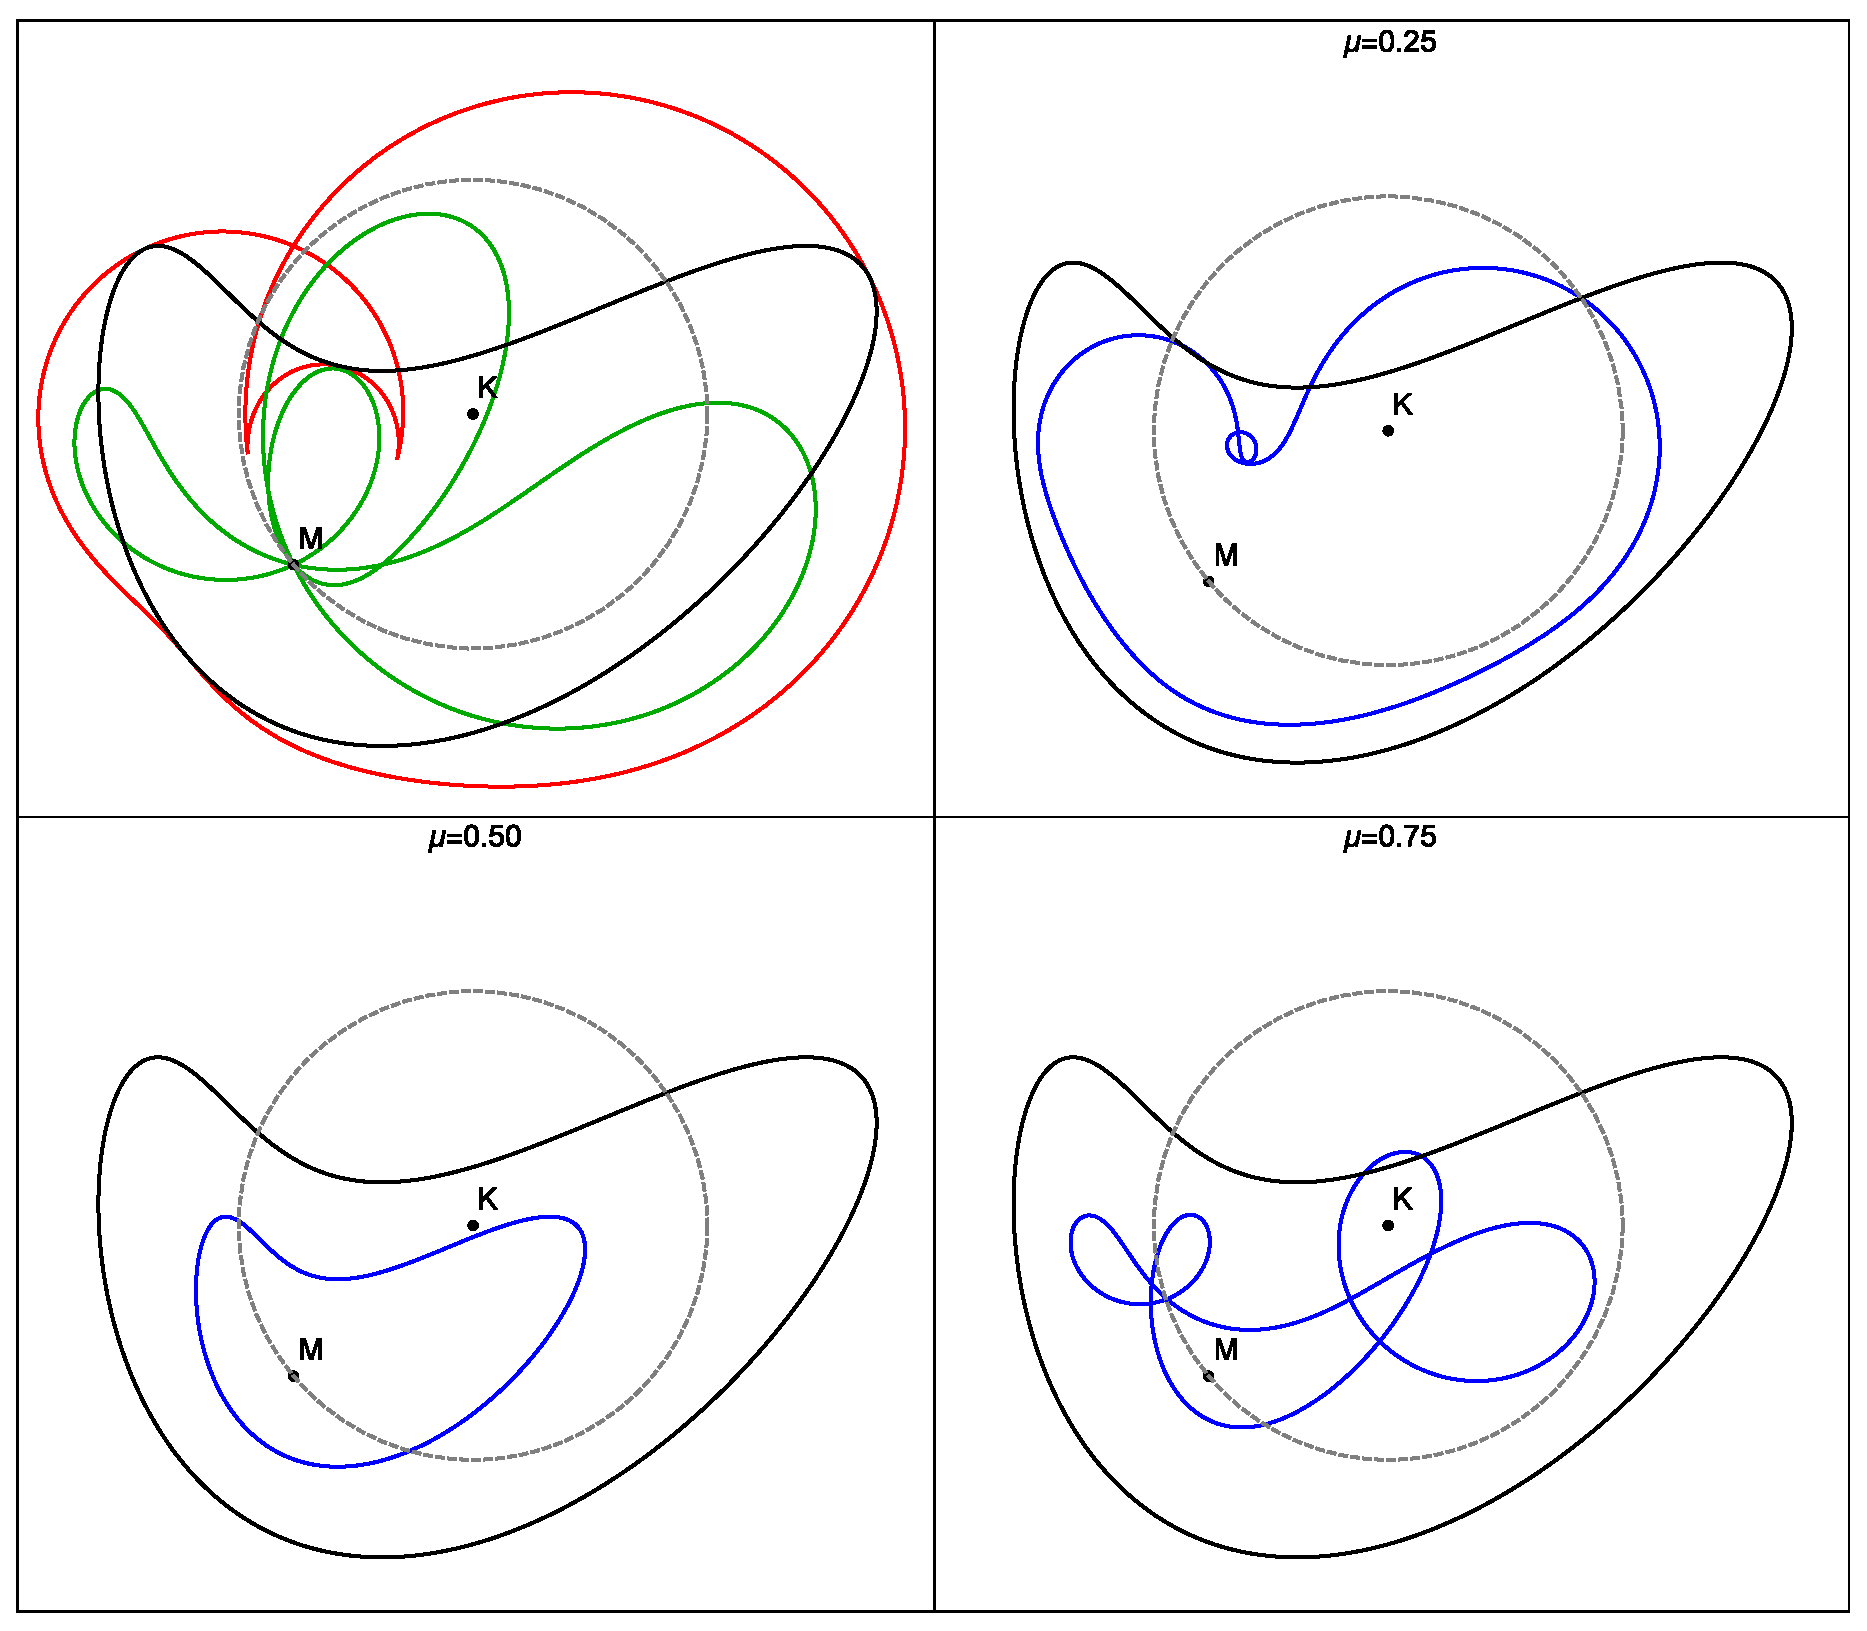
\includegraphics[width=\textwidth]{pics/0070_interpolated_concave.eps}
    \caption{\textbf{Top left}: a generic concave curve $\mathcal{C}$ (black) is shown as well as its curvature centroid $K$ and a circle about it where $M$ lies. Also shown are the pedal (red) and contrapedal (green) curves with respect to $M$. Note their areas are invariant for $M$ anywhere on a circle centered on $K$. \textbf{Top right, bottom left, bottom right}: the interpolated pedal curve (blue) for $\mu=0.25$, $0.5$, and $0.75$, respectively. Its area is also invariant for $M$ on a circle centered on $K$. Notice that at $\mu=0.5$ (bottom left) the interpolated pedal is homothetic (scale of 1/2) to $\mathcal{C}$ and its shape (and area) is independent of the location of $M$. Video of interpolated curve vs $\mu$: \href{
    https://youtu.be/0SW\_tBUeNKg}{\texttt{https://youtu.be/0SW\_tBUeNKg}}. Video of area invariance over circle for various $\mu$: \href{https://youtu.be/gR8Axe823\_M}{\texttt{https://youtu.be/gR8Axe823\_M}}}
    \label{fig:interp-concave}
\end{figure}